\documentclass{article}
\usepackage{v-test-paper}
\newenvironment{solution}{\par\noindent\color{red!85!black}$\Rightarrow$\vspace{0em}}{}

\title{\textsc{JEE Advanced 2023 Paper-I\\Physics}}
\date{}


\begin{document}
\maketitle


\begin{enumerate}
    
\begin{enumerate}
    \item In a historical experiment to determine Planck's constant, a metal surface was irradiated with light of different wavelengths. The emitted photoelectron energies were measured by applying a stopping potential. The relevant data for the wavelength (\(\lambda\)) of incident light and the corresponding stopping potential (\(V_0\)) are given below:
    \begin{center}
        \begin{tabular}{ccc}
        \hline
        \(\lambda (\mu m)\) & \(V_0 (Volt)\) \\
        \hline
        0.3 & 2.0 \\
        0.4 & 1.0 \\
        0.5 & 0.4 \\
        \hline
        \end{tabular}
    \end{center}
    Given that \( c = 3 \times 10^8 m\ s^{-1} \) and \( e = 1.6 \times 10^{-19} C \), Planck's constant (in units of J s) found from such an experiment is
    \begin{tasks}(2)
        \task \( 6.0 \times 10^{-34} \)
        \task \( 6.4 \times 10^{-34} \)
        \task \( 6.6 \times 10^{-34} \)
        \task \( 6.8 \times 10^{-34} \)
    \end{tasks}
\end{enumerate}

    
\item In the arrangement of Fig. 1.9 the masses \( m_0 \), \( m_1 \), and \( m_2 \) of bodies are equal, the masses of the pulley and the threads are negligible, and there is no friction in the pulley. Find the acceleration \( w \) with which the body \( m_0 \) comes down, and the tension of the thread binding together the bodies \( m_1 \) and \( m_2 \), if the coefficient of friction between these bodies and the horizontal surface is equal to \( k \). Consider possible cases.
    \begin{center}
        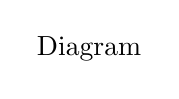
\begin{tikzpicture}
            \node at (0, 0) {Diagram};
        \end{tikzpicture}
    \end{center}

    
\begin{enumerate}
    \item A current carrying wire heats a metal rod. The wire provides a constant power (P) to the rod. The metal rod is enclosed in an insulated container. It is observed that the temperature (T) in the metal rod changes with time (t) as
    \[
    T(t) = T_0(1 + \beta t)^{\frac{1}{4}},
    \]
    where \(\beta\) is a constant with appropriate dimension while \(T_0\) is a constant with dimension of temperature. The heat capacity of the metal is;
        \begin{tasks}(2)
            \task \(\frac{4P(T(t)-T_0)^3}{\beta^4 T_0}\)
            \task \(\frac{4P(T(t)-T_0)^4}{\beta^4 T_0^5}\)
            \task \(\frac{4P(T(t)-T_0)^2}{\beta^4 T_0^3}\)
            \task \(\frac{4P(T(t)-T_0)}{\beta^4 T_0^2}\)
        \end{tasks}
\end{enumerate}

    
\item A point moves rectilinearly in one direction. Fig. 1.1 shows the distance \( s \) traversed by the point as a function of the time \( t \).
    \begin{center}
        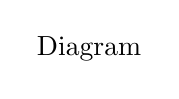
\begin{tikzpicture}
            \node at (0, 0) {Diagram}; % Replace this with the actual TikZ code for the diagram.
        \end{tikzpicture}
    \end{center}
Using the plot find:
\begin{itemize}
    \item the average velocity of the point during the time of motion;
    \item the maximum velocity;
    \item the time moment \( t_0 \) at which the instantaneous velocity is equal to the mean velocity averaged over the first \( t_0 \) seconds.
\end{itemize}

    \item A disc of mass \( m = 50 \) g slides with the zero initial velocity down an inclined plane set at an angle \( \alpha = 30^\circ \) to the horizontal; having traversed the distance \( l = 50 \) cm along the horizontal plane, the disc stops. Find the work performed by the friction forces over the whole distance, assuming the friction coefficient \( k = 0.15 \) for both inclined and horizontal planes.
    \begin{center}
        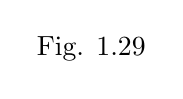
\begin{tikzpicture}
            \node at (0, 0) {Fig. 1.29};
        \end{tikzpicture}
    \end{center}\begin{solution}
    \begin{center}
        \begin{tikzpicture}
            \pic at (0, 0) {frame=3cm};
        \end{tikzpicture}
    \end{center}

    \begin{align*}
        \intertext{Let \(s\) be the distance covered by the disk along the incline, from the equation of increment of mechanical energy of the disk in the field of gravity: \(\Delta T + \Delta U - A_{fr}\)}
        0 + (-mgs\sin\alpha) &= -kmg\cos\alpha \cdot s - kmgl\\
        \intertext{or}
        s &= \dfrac{kl}{\sin\alpha - k\cos\alpha} \tag{1}
        \intertext{Hence the sought work}
        A_{fr} &= -kmg[s \cos\alpha + l]\\
        A_{fr} &= -\dfrac{klmg}{1 - k \cos\alpha} \quad \text{(using Eq. 1)}
        \intertext{On putting the values}
        A_{fr} &= -0.05 \, \text{J}
    \end{align*}
\end{solution}
    \item Two bars of masses $m_1$ and $m_2$ connected by a non-deformed light spring rest on a horizontal plane. The coefficient of friction between the bars and the surface is equal to $k$. What minimum constant force has to be applied in the horizontal direction to the bar of mass $m_1$ in order to shift the other bar?
\begin{solution}
    \begin{center}
        \begin{tikzpicture}
            \pic at (0, 0) {frame=3cm};
        \end{tikzpicture}
    \end{center}

    \begin{align*}
        \intertext{Let \(x\) be the compression in the spring when the bar \(m_2\) is about to shift. Therefore at this moment spring force on \(m_2\) is equal to the limiting friction between the bar \(m_2\) and horizontal floor. Hence}
        \kappa x &= km_2 g \quad \text{[where \(\kappa\) is the spring constant (say)]} \quad \tag{1}
        \intertext{For the block \(m_1\) from work-energy theorem:}
        A &= \Delta T = 0 \text{ for minimum force. (A here includes the work done in stretching the spring.)}
        \intertext{So,}
        Fx - \dfrac{1}{2} \kappa x^2 - km_1 g x &= 0 \quad \text{or} \quad \kappa \dfrac{x}{2} = F - km_1 g \quad \tag{2}
        \intertext{From Eqs. (1) and (2),}
        F &= kg \left(m_1 + \dfrac{m_2}{2}\right)
    \end{align*}
\end{solution}

    
\begin{enumerate}
    \item Two loudspeakers \(M\) and \(N\) are located 20 m apart and emit sound at frequencies 118 Hz and 121 Hz, respectively. A car is initially at a point \(P\), 1800 m away from the midpoint \(Q\) of the line \(MN\) and moves towards \(Q\) constantly at 60 km/hr along the perpendicular bisector of \(MN\). It crosses \(Q\) and eventually reaches a point \(R\), 1800 m away from \(Q\). Let \(v_P\), \(v_Q\) and \(v_R\) be the beat frequencies measured by a person sitting in the car at time \(t\). Let \(v(t)\) represent the beat frequency measured by a person sitting in the car at time \(t\). The speed of sound in air is 330 m s\(^{-1}\). Which of the following statement(s) is(are) true regarding the sound heard by the person?
        \begin{tasks}(1)
            \task \(v_P + v_R = 2 v_Q\)
            \task The rate of change in beat frequency is maximum when the car passes through \(Q\)
            \task The plot below represents schematically the variation of beat frequency with time (with a labeled diagram indicating points \(P\), \(Q\), and \(R\).)
            \task The plot below represents schematically the variation of beat frequency with time (with a labeled diagram indicating points \(P\), \(Q\), and \(R\).)
        \end{tasks}
\end{enumerate}
\begin{center}
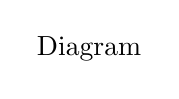
\begin{tikzpicture}
\node {Diagram};
\end{tikzpicture}
\end{center}

    
\item A spherical metal shell A of radius $R_A$ and a solid metal sphere B of radius $R_B$ ($R_B < R_A$) are kept far apart and each is given charge $`+Q'$. Now they are connected by a thin metal wire. Then
    \begin{tasks}(2)
        \task $E_{\text{inside}}^A = 0$
        \task $Q_A > Q_B$
        \task $\frac{\sigma_A}{\sigma_B} = \frac{R_B}{R_A}$
        \task $E_{\text{on surface}}^A < E_{\text{on surface}}^B$
    \end{tasks}

    
\begin{enumerate}
\item A ball is thrown from ground at an angle $\theta$ with horizontal and with an initial speed $u_0$. For the resulting projectile motion, the magnitude of average velocity of the ball up to the point when it hits the ground for the first time is $V_1$. After hitting the ground, the ball rebounds at the same angle $\theta$ but with a reduced speed of $u_0/\alpha$. Its motion continues for a long time as shown in figure. If the magnitude of average velocity of the ball for entire duration of motion is $0.8 V_1$, the value of $\alpha$ is \_\_\_\_\_\_\_.

\begin{center}
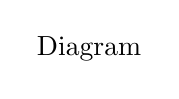
\begin{tikzpicture}
\node {Diagram};
\end{tikzpicture}
\end{center}

\end{enumerate}

    
\item A series R-C circuit is connected to AC voltage source. Consider two cases; (A) when C is without a dielectric medium and (B) when C is filled with dielectric of constant 4. The current $I_R$ through the resistor and voltage $V_C$ across the capacitor are compared in the two cases. Which of the following is/are true?
    \begin{tasks}(2)
        \task $I^A_R > I^B_R$
        \task $I^A_R < I^B_R$
        \task $V^A_C > V^B_C$
        \task $V^A_C < V^B_C$
    \end{tasks}

    
\item A cubical region of side \( a \) has its centre at the origin. It encloses three fixed point charges, \( -q \) at \( (0, -a/4, 0) \), \( +3q \) at \( (0,0,0) \) and \( -q \) at \( (0,+a/4,0) \). Choose the correct option(s).
    \begin{center}
        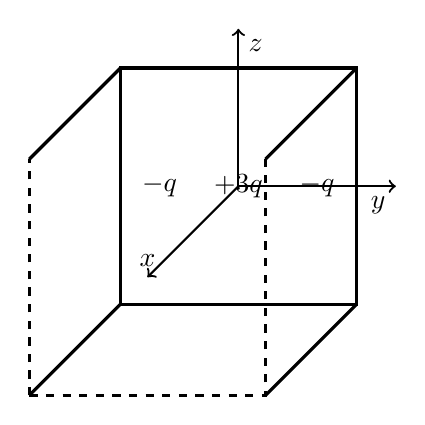
\begin{tikzpicture}
            % Drawing the cube with charges, as a simple representation
            \draw[very thick] (-1.5,-1.5,0) -- (-1.5,1.5,0) -- (1.5,1.5,0) -- (1.5,-1.5,0) -- cycle; % base
            \draw[very thick] (-1.5,-1.5,0) -- (-1.5,-1.5,3);
            \draw[very thick] (-1.5,1.5,0) -- (-1.5,1.5,3);
            \draw[very thick] (1.5,1.5,0) -- (1.5,1.5,3);
            \draw[very thick] (1.5,-1.5,0) -- (1.5,-1.5,3);

            \draw[very thick, dashed] (-1.5,-1.5,3) -- (1.5,-1.5,3) -- (1.5,1.5,3); % top
            \draw[very thick, dashed] (-1.5,-1.5,3) -- (-1.5,1.5,3);

            % Charges
            \node at (-1, 0, 0) { \( -q \) };
            \node at (0, 0, 0) { \( +3q \) };
            \node at (1, 0, 0) { \( -q \) };

            % Axes
            \draw[thick,->] (0,0,0) -- (2,0,0) node[anchor=north east] {\( y \)};
            \draw[thick,->] (0,0,0) -- (0,2,0) node[anchor=north west] {\( z \)};
            \draw[thick,->] (0,0,0) -- (0,0,3) node[anchor=south] {\( x \)};
        \end{tikzpicture}
    \end{center}
    \begin{tasks}(2)
        \task The net electric flux crossing the plane \( x = +a/2 \) is equal to the net electric flux crossing the plane \( x = -a/2 \).
        \task The net electric flux crossing the plane \( y = +a/2 \) is more than the net electric flux crossing the plane \( y = -a/2 \).
        \task The net electric flux crossing the entire region is \( \frac{q}{\varepsilon_0} \).
        \task The net electric flux crossing the plane \( z = +a/2 \) is equal to the net electric flux crossing the plane \( x = +a/2 \).
    \end{tasks}

    \item A horizontal plane with the coefficient of friction \( k \) supports two bodies: a bar and an electric motor with a battery on a block. A thread attached to the bar is wound on the shaft of the electric motor. The distance between the bar and the electric motor is equal to \( l \). When the motor is switched on, the bar, whose mass is twice as great as that of the other body, starts moving with a constant acceleration \( w \). How soon will the bodies collide?\begin{solution}
    \begin{center}
        \begin{tikzpicture}
            \pic at (0, 0) {frame=3cm};
        \end{tikzpicture}
    \end{center}
    
    \begin{align*}
        \intertext{From the Newton’s second law in projection form}
        \text{For the bar,} \quad T - 2 \ k \ m \ g &= (2m) \ w \tag{1}\\
        \text{For the motor,} \quad T - kmg &= mw' \tag{2}\\
        \intertext{Now, from the equation of kinematics in the frame of bar or motor}
        l &= \frac{1}{2} (w + w') \ t^2 \tag{3}\\
        \intertext{From Eqs. (1), (2) and (3) we get on eliminating $T$ and $w'$}
        t &= \sqrt{\frac{2l}{kg + 3w}}
    \end{align*}
\end{solution}
    


OLD MELODIES

\noindent Differentiation | \textbf{123}

\paragraph{Example 6.} The position of a particle moving along \(x\)-axis varies with time \( t \)
according as 
\[
x = t^2 - t + 1
\]
Velocity \( v_x \) and acceleration \( a_x \) of the particles are defined as
\[
v_x = \frac{dx}{dt} \quad \text{and} \quad a_x = \frac{dv_x}{dt}
\]
(i) Find velocity and acceleration at \( t = 1 \).

(ii) When is the velocity of the particle zero?

\noindent \textbf{Solution.} 
\[
v_x = \frac{dx}{dt} = \frac{d(t^2 - t + 1)}{dt} = 2t - 1
\]

\[
a_x = \frac{dv_x}{dt} = \frac{d(2t - 1)}{dt} = 2
\]

(i) At \( t = 1 \),
\[
v_x = 2 \times 1 - 1 = 1
\]
\[
a_x = 2
\]

(ii) \( v_x = 0 \)
\begin{align*}
\Rightarrow & \quad 2t - 1 = 0 \\
\Rightarrow & \quad t = \frac{1}{2} 
\end{align*}
Hence, \( v_x = 0 \) at \( t = \frac{1}{2} \)

\paragraph{Example 7.} The position of a particle moving in \( xy \)-plane varies with time \( t \)
according as 
\[
x = t + 1, \quad y = t - t^2
\]
Find \(\frac{dy}{dx}\)

\noindent \textbf{Solution.} 
\[
\frac{dy}{dx} = \frac{dy}{dt} \bigg/ \frac{dx}{dt} = \frac{d(t - t^2)}{dt} \bigg/ \frac{d(t + 1)}{dt} = \frac{(1 - 2t)}{1} = 1 - 2t
\]

\paragraph{Example 8.} The velocity \( v_x \) of a particle moving along \( x \)-axis varies with its
position \( x \) according as \( v_x = x^2 + 2x - 4 \)

Find acceleration \( a_x \) of the particle as a function of its position \( x \). Velocity \( v_x \) and acceleration \( a_x \) of the particle are defined as \( v_x = \frac{dx}{dt}, \, a_x = \frac{dv_x}{dt} \) where \( t \) denotes time

\noindent \textbf{Solution.} 
\[
a_x = \frac{dv_x}{dt}
\]
\[
\frac{dv_x}{dx} \cdot \frac{dx}{dt} = v_x \cdot \frac{dv_x}{dx}
\]
\[
a_x = (x^2 + 2x - 4) \cdot \frac{d (x^2 + 2x - 4)}{dx}
\]
\[
a_x = (x^2 + 2x - 4)(2x + 2)
\]
\[
a_x = 2 (x + 1) (x^2 + 2x - 4)
\]


    
\begin{enumerate}
    \item An optical bench has 1.5 m long scale having four equal divisions in each cm. While measuring the focal length of a convex lens, the lens is kept at 75 cm mark of the scale and the object pin is kept at 45 cm mark. The image of the object pin on the other side of the lens overlaps with image pin that is kept at 135 cm mark. In this experiment, the percentage error in the measurement of the focal length of the lens is \_\_\_\_\_\_.
\end{enumerate}

    
\begin{enumerate}
    \item A train S1, moving with a uniform velocity of 108 km/h, approaches another train S2 standing on a platform. An observer O moves with a uniform velocity of 36 km/h towards S2, as shown in figure. Both the trains are blowing whistles of same frequency 120 Hz. When O is 600 m away from S2 and distance between S1 and S2 is 800 m, the number of beats heard by O is \_\_\_\_\_\_\_\_\_. \\
    [Speed of the sound = 330 m/s]
    \begin{center}
        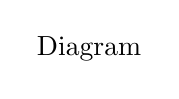
\begin{tikzpicture}
            \node {Diagram};
        \end{tikzpicture}
    \end{center}
\end{enumerate}

    \item From the photoelectric effect experiment, following observations are made. Identify which of these are correct.
    \begin{tasks}(1)
        \task The stopping potential depends only on the work function of the metal.
        \task The saturation current increases as the intensity of incident light increases.
        \task The maximum kinetic energy of a photo electron depends on the intensity of the incident light.
        \task Photoelectric effect can be explained using wave theory of light.
    \end{tasks}
    
Choose the correct answer from the options given below:
\begin{tasks}(2)
        \task B, C only
        \task A, C, D only
        \task A, B, D only
        \task B only
    \end{tasks}
     1. A stationary tuning fork is in resonance with an air column in a pipe. If the tuning fork is moved with a speed of \(2\text{ m s}^{-1}\) in front of the open end of the pipe and parallel to it, the length of the pipe should be changed for the resonance to occur with the moving tuning fork. If the speed of sound in air is \(320\text{ m s}^{-1}\), the smallest value of the percentage change required in the length of the pipe is _____.

\begin{center}
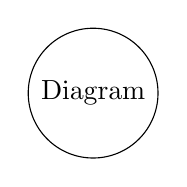
\begin{tikzpicture}
  \node [draw, shape=circle] {Diagram};
\end{tikzpicture}
\end{center}
\end{enumerate}

\pagebreak
\begin{center}
    \textsc{2023, Paper-I}
\end{center}

\begin{center}
\texttt{Answer Key}
\begin{multicols}{5}
\begin{enumerate}
\item (b)
\item (b)
\item (a)
\item (b)
\item (d)
\item (b)
\item (c)
\item (a), (b)
\item (c)
\item (a), (b), (c), (d)
\end{enumerate}
\end{multicols}
\end{center}



\end{document}
